%%% Local Variables:
%%% mode: latex
%%% TeX-master: t
%%% End:

\newpage
\subsection{Use Case Modeling}

A use case diagram is a graphical depiction of a user's possible interactions with a system. A use case diagram shows various use cases and different types of users the system has and will often be accompanied by other types of diagrams as well.
In Devault the user can upload, download, share, delete, sort, and search files. Also the user can connect and disconnect their blockchain wallet.

\subsubsection{Use Case Diagram}

%%% Local Variables:
%%% mode: latex
%%% TeX-master: t
%%% End:
\namedfigure
{!htbp}
{img:dAppUscsDig}
{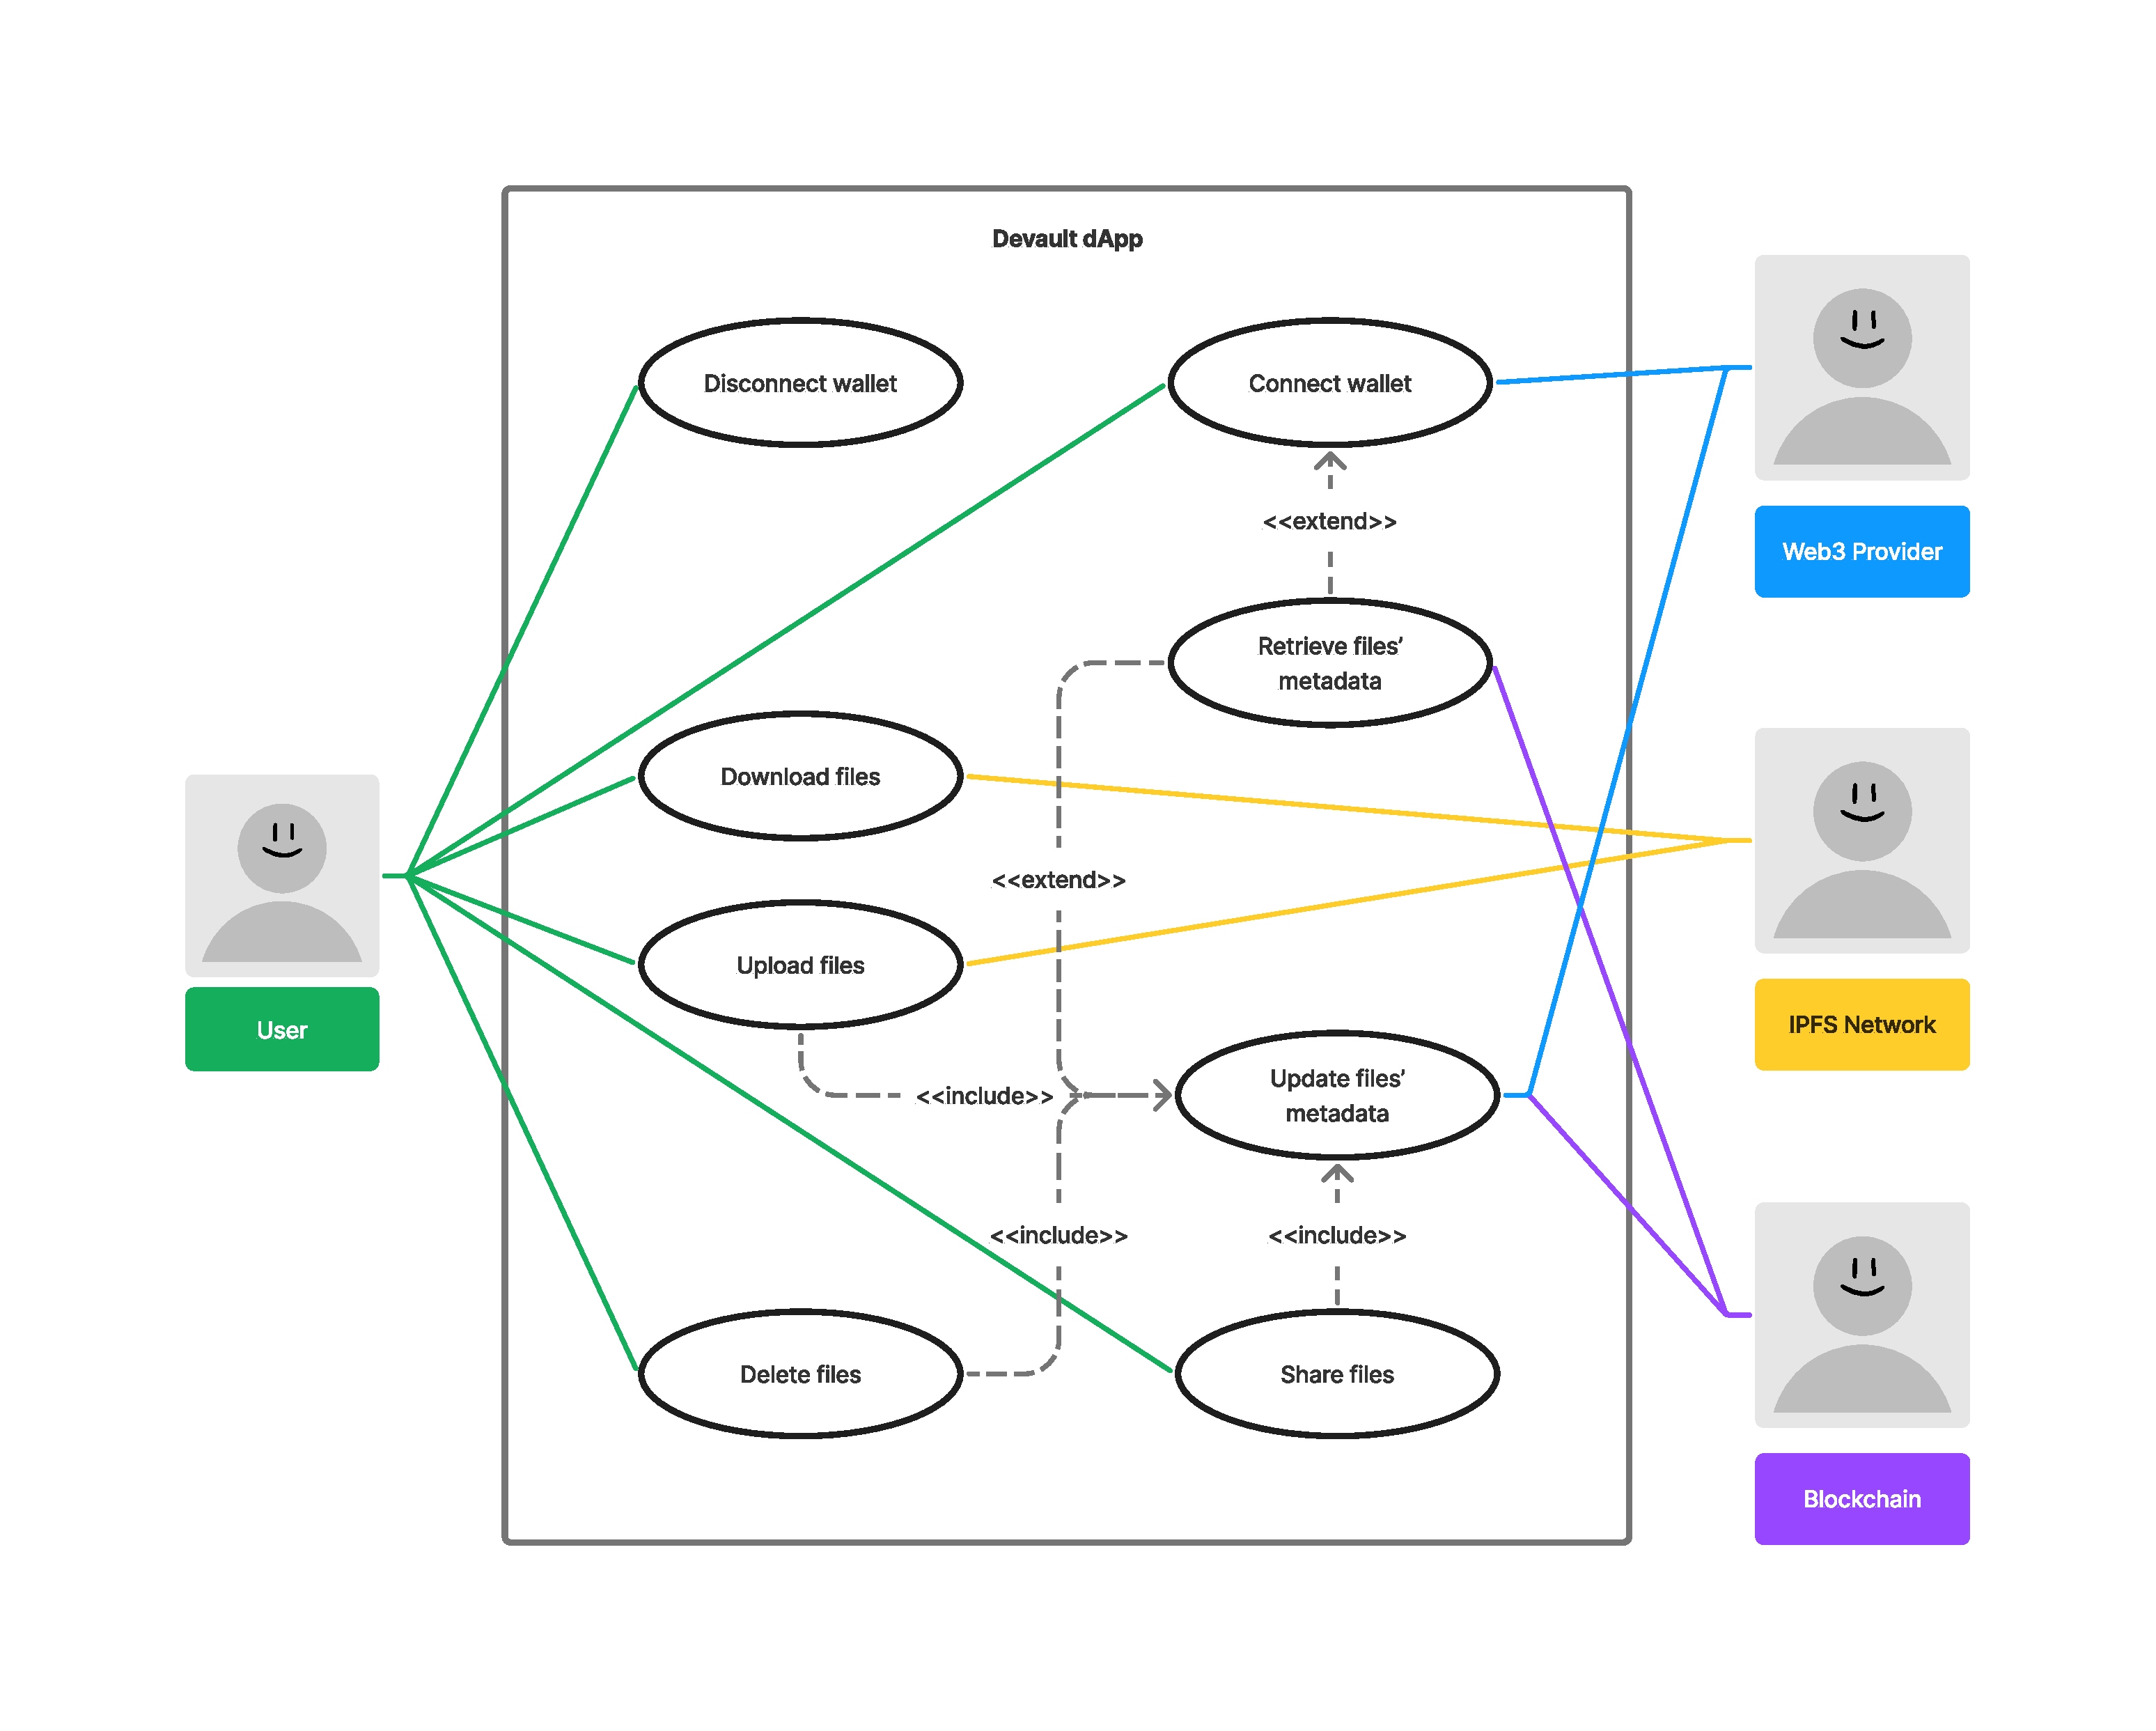
\includegraphics[width=\textwidth]{dapp_uscs_dig.pdf}}
{dApp use case diagram.}


\subsubsection{Use Case Model}

\begin{longtable}{p{0.20\linewidth} | p{0.75\linewidth}}
  \caption{Use case 1: Connecting wallet}
  \label{tab:useCaseConnect}
  \\\toprule
  ID & UC\_1
  \\\midrule
  Title & \textbf{Connecting wallet}
  \\\hline
  Description & The user can connect with their Ethereum wallet to use the system.
  \\\hline
  Primary Actor & User.
  \\\hline
  Pre-Conditions & {
    \begin{itemize}
    \item The user must have internet connection.
    \item The user navigates to \url{devault.vercel.app} or any other instance.
    \end{itemize}
  }\vspace*{-\baselineskip}
  \\\hline
  Main Success Scenario & {
    \begin{enumerate}
    \item The user clicks the connect wallet button.
    \item The user confirms the connection.
    \item The system then will retrieve the files from that account.
    \end{enumerate}
  }\vspace*{-\baselineskip}
  \\\bottomrule
\end{longtable}

\begin{longtable}{p{0.20\linewidth} | p{0.75\linewidth}}
  \caption{Use case 2: Uploading files}
  \label{tab:useCaseUpload}
  \\\toprule
  ID & UC\_2
  \\\midrule
  Title & \textbf{Uploading files}
  \\\hline
  Description & The user can upload files or folders to the system.
  \\\hline
  Primary Actor & User.
  \\\hline
  Pre-Conditions & {
    \begin{itemize}
    \item UC\_1
    \end{itemize}
  }\vspace*{-\baselineskip}
  \\\hline
  Main Success Scenario & {
    \begin{enumerate}
    \item The user navigates to the vault tab.
    \item The user clicks on the upload button and picks a file or folder to upload.
    \item The user enters a password to encrypt the files.
    \item The system then will encrypt the files, store their metadata in the blockchain, and upload the encrypted files to the \gls{p2p g} network.
    \end{enumerate}
  }\vspace*{-\baselineskip}
  \\\bottomrule
\end{longtable}

\begin{longtable}{p{0.20\linewidth} | p{0.75\linewidth}}
  \caption{Use case 3: Downloading files}
  \label{tab:useCaseDownload}
  \\\toprule
  ID & UC\_3
  \\\midrule
  Title & \textbf{Downloading files}
  \\\hline
  Description & The user can download files or folders from the system.
  \\\hline
  Primary Actor & User.
  \\\hline
  Pre-Conditions & {
    \begin{itemize}
    \item UC\_1
    \end{itemize}
  }\vspace*{-\baselineskip}
  \\\hline
  Main Success Scenario & {
    \begin{enumerate}
    \item The user navigates to the vault tab.
    \item The user selects the files they need to download.
    \item The user enter a password to decrypt the files.
    \item The system then will decrypt the files and download them.
    \end{enumerate}
  }\vspace*{-\baselineskip}
  \\\bottomrule
\end{longtable}

\begin{longtable}{p{0.20\linewidth} | p{0.75\linewidth}}
  \caption{Use case 4: Sharing files}
  \label{tab:useCaseShare}
  \\\toprule
  ID & UC\_4
  \\\midrule
  Title & \textbf{Sharing files}
  \\\hline
  Description & The user can share files or folders with other users.
  \\\hline
  Primary Actor & User.
  \\\hline
  Pre-Conditions & {
    \begin{itemize}
    \item UC\_1
    \end{itemize}
  }\vspace*{-\baselineskip}
  \\\hline
  Main Success Scenario & {
    \begin{enumerate}
    \item The user navigates to the vault tab.
    \item The user selects the files they need to share.
    \item The user clicks the share button.
    \item The user will be prompted to enter the addresses to share the file.
    \item The system then will share the files with these addresses.
    \end{enumerate}
  }\vspace*{-\baselineskip}
  \\\bottomrule
\end{longtable}

\begin{longtable}{p{0.20\linewidth} | p{0.75\linewidth}}
  \caption{Use case 5: Deleting files}
  \label{tab:useCaseDelete}
  \\\toprule
  ID & UC\_5
  \\\midrule
  Title & \textbf{Deleting files}
  \\\hline
  Description & The user can Delete files or folders form the system.
  \\\hline
  Primary Actor & User.
  \\\hline
  Pre-Conditions & {
    \begin{itemize}
    \item UC\_1
    \end{itemize}
  }\vspace*{-\baselineskip}
  \\\hline
  Main Success Scenario & {
    \begin{enumerate}
    \item The user navigates to the vault tab.
    \item The user selects the files they need to delete.
    \item The user clicks the delete button.
    \item The user will be prompted to confirm the deletion process.
    \item The system then will delete the files with form the user address.
    \end{enumerate}
  }\vspace*{-\baselineskip}
  \\\bottomrule
\end{longtable}

\begin{longtable}{p{0.20\linewidth} | p{0.75\linewidth}}
  \caption{Use case 6: Disconnecting wallet}
  \label{tab:useCaseDisconnect}
  \\\toprule
  ID & UC\_6
  \\\midrule
  Title & \textbf{Disconnecting wallet}
  \\\hline
  Description & The user can disconnect their Ethereum wallet from the system.
  \\\hline
  Primary Actor & User.
  \\\hline
  Pre-Conditions & {
    \begin{itemize}
    \item UC\_1
    \end{itemize}
  }\vspace*{-\baselineskip}
  \\\hline
  Main Success Scenario & {
    \begin{enumerate}
    \item The user clicks the disconnect wallet button.
    \item The system will log this user out.
    \end{enumerate}
  }\vspace*{-\baselineskip}
  \\\bottomrule
\end{longtable}
